\documentclass[a4paper,12pt]{article}
\usepackage[top=3cm, bottom=3cm, left=3cm, right=3cm]{geometry}	%dimension de la feuille
\usepackage[utf8]{inputenc}%codage linux
\usepackage[T1]{fontenc}%les fontes
\usepackage[french]{babel}%caractères français
\usepackage{amsmath}
\usepackage{amssymb}
\usepackage{mathrsfs}
\usepackage{hyperref}%liens pdf
\usepackage{listings}%pour mettre du code
\usepackage{color}%pour la couleur dans le code
\usepackage{graphicx}%pour \includegraphics
\usepackage{float}
\usepackage{longtable}
\usepackage[table]{xcolor}
\lstset{breaklines=true}
\usepackage{verbatim}
\usepackage{array}
\usepackage{svg}

\usepackage{pdfpages}

%%%%%%%%%%%%%%%%%%%% Presentation %%%%%%%%%%%%%%%%%%%
\title{\huge Interactions Homme-Machine Évoluées\\Rapport\\Sujet : Stance detection sur tweeter}
\author{Ingrid FIQUET\\Morgane LEGROS\\Florian MARTIN\\Thibault THÉOLOGIEN}
\date{\today}


\begin{document}
	\begin{titlepage}
		\vfill
		\begin{figure}
			
\includegraphics[scale=0.3]{img/logo_insa_rouen.png}
		\end{figure}

		\maketitle


    \begin{center}
    \LARGE
      \addvspace{10mm}
      À l'attention d'Alexandre Pauchet.
    \end{center}

		\vfill
		\noindent \hrulefill

	\end{titlepage}


%%%%%%%%%%%%%%%%%%%% Corps %%%%%%%%%%%%%%%%%%%

\newpage
\tableofcontents{}

\newpage
\part{Introduction}
		\par Ce document concerne la présentation de réalisation du projet dans le cadre de l'EC Interaction Homme-Machines Évoluées.  
	\par L'objectif de ce projet est de réaliser une analyse de tweet afin d'en extraire le stance, c'est à dire déterminer si l'auteur du tweet était 'POUR', 'CONTRE' ou 'NEUTRE' via à vis d'un sujet donnée.\\ 
	\par Nous avions à notre disposition deux jeux de données concenant les informations suivantes : le tweet, le sujet du tweet, l'opinion toward (c'est à dire si le tweet à un lien direct ou non avec le sujet), le sentiment (positif, négatif ou neutre) et le stance du tweet (pour, contre, neutre). 
	\par Notre choix d'implémentation pour notre sujet a été de réaliser 3 briques logicielles permettant chacune de déterminer, le sentiment du tweet, l'opinion toward et le stance. \\
	\par Dans un premier temps nous vous présenterons la conception réalisé sur ce sujet et ensuite nous vous détaillerons les choix et le résultat des implémentations réalisés pour nos 3 briques logicielles.

	\newpage
% Expliquer notre idée et les différentes étapes

\part{Conception}

\section{Conception Préliminaire}
	\par Cette partie présente la conception préliminaire qui a été réalisée.

	%\section{Diagramme de modèle du domaine}


	%\section{Diagramme du flux de traitement des données}


\section {Diagramme de la couche machine learning}
\begin{figure}[h!]
	\centerline{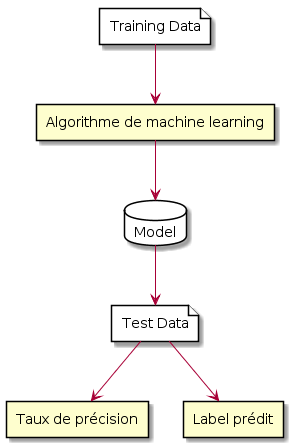
\includegraphics[scale=0.8]{img/diagML.png}}
	\caption{Diagramme des méthodes d'apprentissage}
\end{figure}


\section {Diagramme Sentiment Analysis}

\begin{figure}[h!]
	\centerline{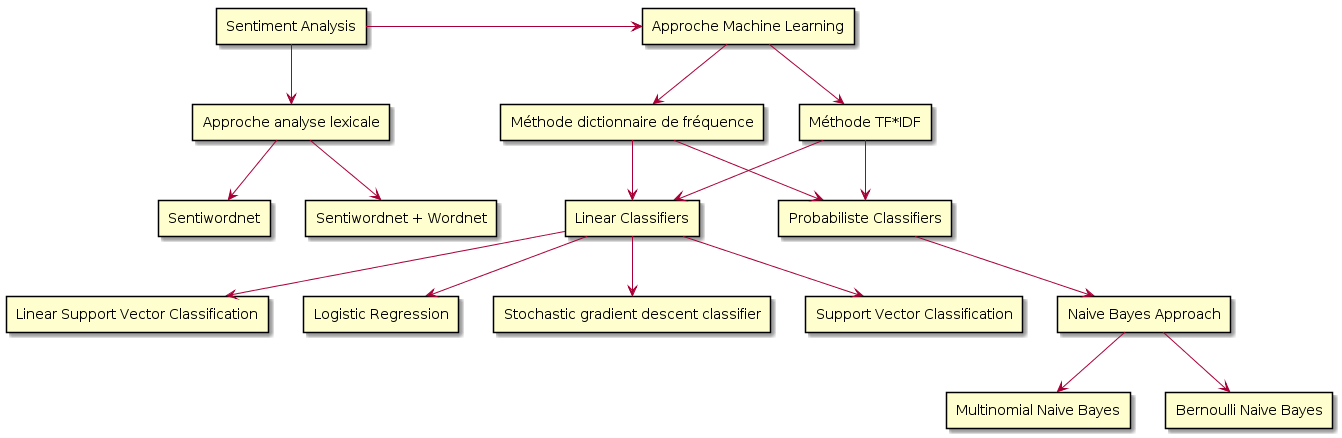
\includegraphics[scale=0.4]{img/DiagSentimentAnalysis.png}}
	\caption{Diagramme général de la brique Sentiment Analysis}
\end{figure}


\begin{figure}[h!]
	\centerline{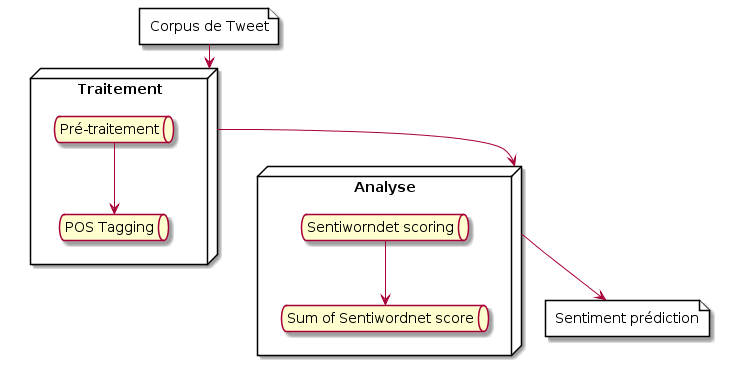
\includegraphics[scale=0.6]{img/DIagSentiwordnet.png}}
	\caption{Diagramme de la méthode de detection de sentiment par sentiwordnet}
\end{figure}
	\newpage


\section{Conception Détaillée}
	\par La conception détaillée consiste à détailler par package les éléments. Concrètement, il s’agit principalement de préciser les attributs et méthodes de classe de toutes les classes participantes et de les regrouper dans un diagramme de classes.

	\subsection{Diagrammes de classes}


	\newpage


\newpage
\part{Implémentation}
	\par Dans cette partie nous allons ainsi vous présenter les trois briques logicielles réalisé pour ce projet et les méthodes de pré-traitement réalisés :

\begin{itemize}
	\item Pré-traitement : formatage des données
	\item Détermination du sentiment du tweet
	\item Détermination de l'opinion towards
	\item 
\end{itemize}

\section{Chargement des données}

Lors de l'étude des données, ne nous sommes rendu compte que le jeu de données d'apprentissage et de test ne comportent pas le même nombre de ". En effet, les tweets concernant le sujet "Donald Trump" ont été ajouté dans le jeu de test.

N'étant pas dans les conditions réelles de la compétition, nous avons décidé de fusionner l'ensemble des datasets afin de les redécouper de manière aléatoire en trois ensembles, l'un d'apprentissage, l'un de test pour tester les différents modèles, et l'un de "validation" \textbf{utilisé une seule fois} dans notre projet pour la prédiction.


\section{Formatage des données}
\par Afin d'améliorer les performances des différents blocs de cette implémentation, nous avons choisi de formater au mieux les données. Uniquement les tweets sont concernés pas ce formatage.

\par Plusieurs méthodes ont été appliquées:
\begin{itemize}
  \item transformation en minuscule de tous les caractères en majuscule.
  \item suppression du hashag \#semst présent à la fin de chaque tweet, et n'apportant aucun caractère informatif au tweets.
  \item remplacement des symboles pouvant être exprimés par des mots en ledit mot. Par exemple, au symbole \% correspond le mot "percent", au symbole \& le mot "and", ...
  \item suppression de tous les symboles ne pouvant pas être exprimés pas des mots, en particulier les symboles de ponctuation.
  \item transformation des formes contractées en leur forme étendue. Par exemple, à "ma'am" correspond le mot "madam", à "I'm" les mots "I am".
  \item transformation des nombres en le mot "number". En effet, la valeur exprimée n'a pas d'influence sur le sens du tweet.
  \item transformation des mentions (utilisation du symbole @) d'utilisateurs, en le mot "someone". Dans certains contextes, la valeur de cette mention pourrait être intéressante (dans le cas ou on arriverait à déterminer si cette mention a une valeur positive ou non par exemple), mais de part l'implémentation que nous avons choisi, ce formatage est plus pertinent, et améliore l'apprentissage du bloc "Opinion towards" detection.
  \item transformation de tous les verbes en leur forme infinitive.
\end{itemize}

\par Quelques autres formatages des tweets pourraient être pertinents dans le cadre de ce projet:
\begin{itemize}
  \item si plusieurs mots ont un synonyme en commun, il pourrait s'avérer judicieux de remplacer lesdits mots par ce synonyme. Ainsi, nous réduisons le dictionnaire de mots utilisés, et pouvons améliorer l'apprentissage du bloc "Opinion towards" detection.
  \item il est compliqué d'extraire le sens des hashags utilisés dans les tweets, cependant il correspondent régulièrement à un groupe de mots collés. Ainsi un hashag comme \#NetNeutrality pourrait être décomposé en deux mots, "net" et "neutrality".
  \item transformation des mots au pluriel en leur forme au singulier. En effet, ils seront interprétés comme étant des mots différents par le bloc "Opinion towards" detection, alors qu'ils n'influent pas sur sens général du tweet.
  \item suppression des répétitions de mots.
\end{itemize}
Certains formatage appliqués ne sont pas forcément des plus précis, et pourraient être améliorés. Par exemple, dans le cas du remplacement des contractions en mots, il est difficile de déterminer si "he's" correspond à "he is" ou "he has".

\section{Sentiment analysis}

\par Concernant la partie détection de sentiment l'objectif est de déterminer si le tweet est "positif", "neutre" ou "négatif". 
\par Pour déterminer la méthode la plus efficace nous avons réaliser une comparaison de plusieurs méthodes :

\begin{itemize}
	\item Étude du sentiment des Tweets à l'aide de la polarité positive, négative et neutre de chaque mot des Tweets via l'utilisation de Sentiwordnet.
	\item Étude du sentiment des Tweets à l'aide de la polarité positive, négative et neutre de chaque mot des Tweets via l'utilisation de Sentiwordnet et de Wordnet.
	\item Détermination du sentiment des Tweets à l'aide de classifier.
\end{itemize}

\subsection{Sentiwordnet}
\par Sentiwordnet est un dictionnaire de mots de référence avec lequel on va travailler dans cette partie.
\par Sentiwordnet permet d'obtenir des scores entre 0 et 1 informant de la forte positivité ou de la forte négativité d'un mot donné. \\


\par \textbf{Principe :} \\
\par Prendre une liste de tweets en entrée. Pour chacun des tweets on va sommer les scores de positivité ainsi que les scores de négativité de tous les mots du tweets. Pour obtenir le score de polarité final du tweet on va soustraire le score de négativité au score de positivité. \\

\par \textbf{Étape de la méthode :} \\
\begin{itemize}
	\item Pré-traitement : Retrait des mots de liaison, déterminant, ponctuation, symbole qui n'ont pas d'impact dans la détermination de la polarité des mots.	 \\
	\item Part Of Speech Tagging : Utilisation de la librairie nltk (Natural Language Toolkit) afin de tagger chaque mots des tweets par leur description grammatical tel que NN pour "nom" ou JJ pour "adjectif". Le but de faire ça dans cette méthode et de pouvoir filtrer les catégories de mots que l'on va donner en entrée de Sentiwordnet pour déterminer leur polarité dans le but d'avoir un meilleur résultat en étudiant les catégories les plus pertinentes. Nous avons donc choisi d'étudier les scores de positivité et de négativité des groupes NN (noms), JJ (adjectifs), VB (verbe), RB (adverbe). \\
	\item Calcul du sentiments de tous les mots retenus dans un tweet pour obtenir la polarité moyenne du tweet. \\
	\item Si le score final du tweet est positif alors la prédiction du tweet est 'positif', si le score est négatif on retourne 'négatif' et si le score vaut 0 on retourne 'neutre'. \\
\end{itemize}

\par \textbf{Résultats :} \\

\begin{table}[h!]
\centering
\caption{Résultats Sentiwordnet}
\label{my-label}
\begin{tabular}{|l|l|}
\hline
                   & Taux de bonne prédiction \\ \hline
Sans-prétraitement & 48,9\%                   \\ \hline
Avec-prétraitement & 54,6\%                   \\ \hline
\end{tabular}
\end{table}



\subsection{Wordnet}

\par L'objectif dans cette méthode est d'utiliser un autre dictionnaire pour étudier la polarité des mots des tweets car le dictionnaire Sentiwordnet possède un lexique restreint ne permettant pas de calculer la polarité de tous les mots donc beaucoup ne sont pas étudié. \\

\par L'avantage avec Wordnet c'est que l'on va extraire les mots des tweets et pour tous les mots on va à l'aide de Wordnet récupérer le mot le plus général du mot en entrée. Par exemple grâce à sa reconnaissance de synonyme wordnet va transformer les mots "sorrowful" et "sad" par le mot "unhappy". Ainsi l'avantage ici c'est que l'on va appliquer la même méthode que précédemment avec Sentiwornet pour le calcul de polarité mais grâce à l'utilisation de Wordnet en amont le dictionnaire Sentiwornet pourra calculer le score de davantage de mots car les mots non présent dans ce dictionnaire auront été remplacé par des mots plus basiques bien présent dans Sentiwornet. \\ 

\par Dans la méthode précédente on a pu constater que les pré-traitement étaient utiles donc nous les avons conserver dans cette méthode également. \\

\par\textbf{ Résultats : } 53,19\%

\subsection{Classifiers}

\par Dans cette partie nous allons nous concentrer sur de la prédiction de sentiment à l'aide de classifier. Contrairement aux deux autres partie nous allons avoir besoin de deux jeux de données, un jeu de donnée d'apprentissage et un jeu de donnée de test. Ainsi à partir du jeu d'apprentissage on va construire notre modèle de prédiction et on va prédire sur les données de test. \\

\par Pour l'utilisation de classifier nous nous sommes tourné vers l'utilisation de la librairie scikit-learn et nltk. \\

\par \textbf{Principe : } \\
\par Pour l'apprentissage les classifier nltk fonctionne avec des structures de caractéristiques, dans notre cas avec des dictionnaires associant le nom d'une caractéristique à une valeur. 
\par D'après une étude bibliographique nous nous sommes tourné vers l'étude de Naive Bayes Classifier dans un premier temps puis ensuite sur des classifiers alternatif.  
\par Nous utilisons ce type de classifier basées sur les fréquences de mots associées à chaque étiquette de positif ou négatif. \\

\par Sur le jeu d'apprentissage pour construire le modèle on va utiliser les informations suivantes : \\
\begin{itemize}
	\item Tweet\_train
	\item Sentiment\_train \\
\end{itemize}


\par \textbf{Étape de la méthode :} \\
\begin{itemize}
	\item Étape 1 : Création des dictionnaires de caractéristiques. On va récupérer trois listes contenant tous les tweets dont le sentiment est 'positif', 'négatif' ou 'neutre' et pour chacune des listes on va créer trois nouvelles listes contenant tous les mots relatif à un tweet positive, négatif ou neutre. Pour optimiser l'analyse qui va suivre on ne conservera que les mots de plus de 6 caractères. A partir de l'extraction des mots de chaque labels, on va construire les dictionnaires de caractéristiques nécessaire à l'utilisation des classifiers. \\
	\item Étape 2 : Avec l'utilisation des librairies on va pouvoir construire des classifiers et estimer la précision des classifiers. On va apprendre le modèle sur un set d'apprentissage composait des structures de caractéristiques pour label positif, négatif et neutre d'apprentissage et on va calculer la précision du modèle avec les structures de caractéristiques de test pour label positif, négatif et neutre du jeu de test. \\
\end{itemize}

\par \textbf{Méthode alternative }: \\
\par Dans la méthode décrite précédemment on construisait nous même nos dictionnaires de caractéristiques mais il est possible d'utiliser les outils de librairies pour les remplacer comme la méthode TF*IDF comme méthode de pondération pour obtenir les structures de caractéristiques pour mettre en place les classifier.
\par C'est donc avec la méthode TF*IDF que nous avons également construit nos classifier et que nous avons évaluer le taux de bonne prédictions.

\par \textbf{Résultats :} \\


\begin{table}[h!]
\centering
\caption{Comparaison des taux de bonne prédiction des classifiers selon deux méthodes}
\label{my-label}
\begin{tabular}{|l|l|l|}
\hline
                   & \begin{tabular}[c]{@{}l@{}}Précision des classifiers avec \\ des dictionnaires de caractéristiques manuel\end{tabular} & \begin{tabular}[c]{@{}l@{}}Taux de bonne prédiction\\ avec la méthode TF*IDS\end{tabular} \\ \hline
BernoulliNB        & 66.9\%                                                                                                                 & 71.2\%                                                                                    \\ \hline
MultinomialNB      & 67.1\%                                                                                                                 & 69,2\%                                                                                    \\ \hline
LogisticRegression & 66.8\%                                                                                                                 & 72.7\%                                                                                    \\ \hline
SGDClassifier      & 63,3\%                                                                                                                 & 70,9\%                                                                                    \\ \hline
SVC                & 65\%                                                                                                                   & 65\%                                                                                      \\ \hline
LinearSVC          & 61,6\%                                                                                                                 & 72.1\%                                                                                    \\ \hline
\end{tabular}
\end{table}

\par \textbf{Conclusion :} \\
\par La méthode la plus efficace est la méthode utilisant TD*IDF avec le classifier Regression Logistique. \\


 
\section{"Opinion towards" detection}

\par 

\subsection{Structure du réseau}

\par Nous avons essayé différentes structures de réseaux de neurones afin d'essayer d'obtenir la meilleure prédiction possible.

\par Tout d'abord, nous nous sommes intéressé aux réseaux de neurones récurrents pour effectuer cette tâche. Nous avons donc mis en place un simple réseau avec un LSTM à 100 cellules. Le résultat obtenu (73,65\% de précision sur les données d'apprentissage) montrait que le réseau avait des difficultés à apprendre les données. Pour résoudre ce problème, nous avons essayé l'ajout de dropout mais sans succès, le coût n'arrivait pas à être correctement minimisé entre chaque epoch. Nous avons donc remplacé les cellules LSTM par des cellules RNN simples, ce qui a eu un effet positif sur l'apprentisssage, mais toujours pas satisfaisant. Nous avons ensuite essayé d'inclure des couches de convolution et de maxpooling afin d'appliquer des filtres aux tweets pour améliorer l'apprentissage. Cette configuration nous satisfaisait jusqu'à ce que nous l'intégrions à l'ensemble des autres solutions pour avoir une chaîne de bout en bout. Mais nous nous sommes rendu compte que finalement, les résultats donnés par cette méthode pouvait très facilement se fausser en fonction du jeu de données à prédire. Nous avons donc finalement décidé de retirer les cellules RNN, nous nous sommes donc retrouvé avec un simple réseau convolutionnel.

\begin{figure}
	\centering
	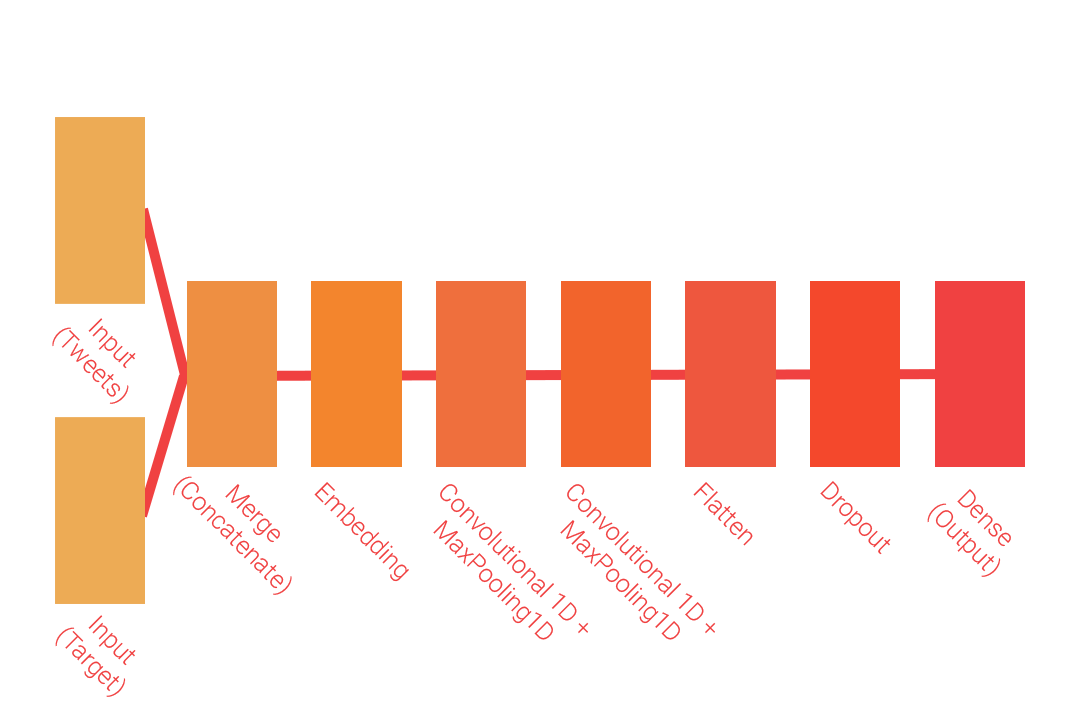
\includegraphics[scale=1.5]{./img/nn.png}
	\caption{Structure du réseau de neurones retenu}
	\label{fig:nn}
\end{figure}

\par Le réseau de neurones retenu (Structure présentée sur la figure \ref{fig:nn}) est donc composé de deux entrées : l'une pour les tweets et l'autre pour la cible de ceux-ci. Ces entrées sont ensuites concaténées en un seul vecteur pour ensuite être passées dans notre réseau convolutionnel qui va appliquer des filtres à notre texte. Enfin, le réseau fait la connection entre la sortie de nos couches convolutionnelles et une couche complètement connectée qui va nous permettre d'obtenir nos prédictions.


\subsection{Apprentissage et résultats}

\begin{table}[h!]
	\centering
	\begin{tabular}{|l|l|l|l|l|l|}
		\hline
		\textbf{lr} & \textbf{$\beta_1$} & \textbf{$\beta_2$} & \textbf{decay} & \textbf{epochs} & \textbf{batch size} \\
		\hline
		0.01 & 0.9 & 0.9 & 0.01 & 10 & 64 \\
		\hline
	\end{tabular}
	\caption{Paramètres retenus pour le réseau.}
	\label{tab:saved_params}
\end{table}

\par L'une des étapes une fois le réseau construit a été de trouver les paramètres pour lesquels celui-ci apprenait le mieux et donnait les meilleurs résultats. Du fait de la multiplicité des paramètres, nous avons décidé de nous concentrer principalement sur les paramètres de l'optimiseur utilisé, c'est-à-dire un optimiseur suivant l'algorithme d'Adam. Les résultats obtenus à la suite d'un script testant divers paramètres, nous avons retenus présentés dans le tableau \ref{tab:saved_params}. Ceux-ci ont été retenus car ils nous permettaient d'obtenir un bon apprentissage des données (99,77\% de précision sur les données d'apprentissage) et donnait un coût minimal (0.0085 avec les données d'apprentissage).

\begin{figure}
	\centering
	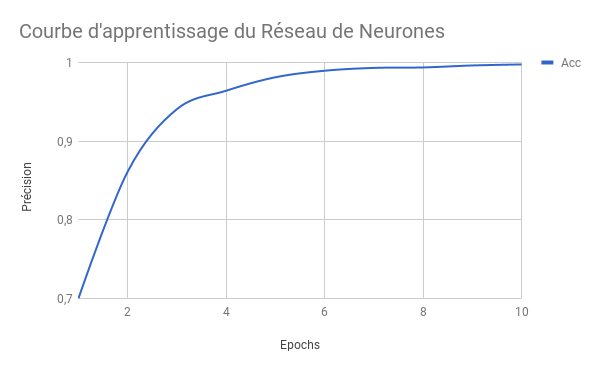
\includegraphics[scale=0.75]{./img/learn_nn_chart.png}
	\caption{Courbe d'apprentissage en fonction des epochs}
	\label{fig:nn_app}
\end{figure}

\par % Commentaire sur la courbe d'apprentissage

\begin{figure}
	\centering
	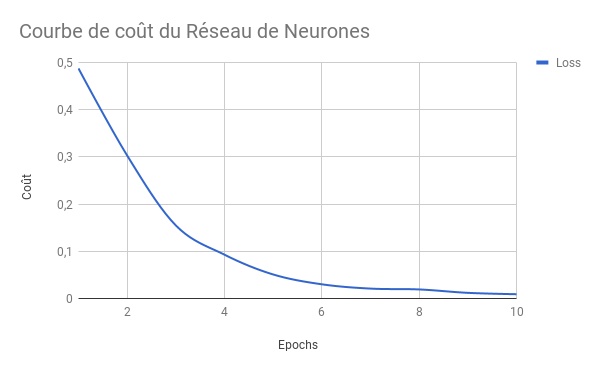
\includegraphics[scale=0.75]{./img/loss_nn_chart.png}
	\caption{Courbe de coût en fonction des epochs}
	\label{fig:nn_loss}
\end{figure}

\par % Commentaire sur la courbe de coût

\par % Commentaire sur le résultat de test (70% -> Peu de données d'apprentissage, classes sous représentées)

% Sources utilisées :
% Convolutional Neural Networks for Sentiment Analysis on Italian Tweets (2016)
% Explaining Recurrent Neural Network Predictions in Sentiment Analysis (2017)

\section{Stance detection}

La partie "Stance detection" consiste à déterminer l'opinion du tweet par rapport au sujet, c'est-à-dire si le tweet est "pour", "contre" ou "neutre" vis à vis du sujet. Cette étape prend en entrée le "Target" (le sujet), le "Sentiment" (positif, négatif ou autre) et l'"Opinion Towards" (le tweet donne un opinion par rapport au sujet, le tweet donne un opinion qui n'a pas de rapport avec le sujet, ou le tweet ne donne pas d'opinion). Ces deux derniers sont déterminés dans les étapes précédentes. Cette dernière étape est donc sensible aux taux d'erreur précédemment obtenus.
La combinaison de ces trois entrées permet de déterminer la "stance". \\

Cette partie est un problème de classification basique, qui prend en entrée trois paramètres qui renvoie une sortie. C'est un problème de classification multi-classe, en effet la sortie se compose de 3 classes : "FAVOR", "AGAINST" et "NONE". \\

\subsection{POC - Traitement des données}

Une première approche a été de tester différentes méthodes de classification usuelles comme SVM et bayes.

Pour cela, un petit traitement sur les données s'impose, effectivement pour utiliser de telles méthodes il est d'abord nécessaire de labelliser les données avec des classes numérotées pour s'abstraire des chaînes de caractères. \\
Dans le jeu de données de train fourni, il y 5 "target" différents, en ce qui concerne le "sentiment" il y a 3 classes possibles et il en est de même pour l'"opinion towards".

En essayant de réaliser une SVM, nous nous sommes rendu compte que dans le jeu de données de test il y avait maintenant 6 "target". En effet, les tweets concernant le sujet "Donald Trump" ont été ajouté. Or, le modèle ne peut pas fonctionner pour un sujet qui n'a pas été appris. 
La solution a dont été de fusionner les ensembles d'apprentissage et de test et de les redécouper de manière aléatoire afin d'obtenir des tweets de l'ensemble des "target" dans l'ensemble d'apprentissage.

\subsection{POC - Test de méthodes de classification}

Tout d'abord, nous avions décidé d'implémenter une méthode de classification bayésienne et une méthode SVM, ensuite il a également été possible d'implémenter d'autres méthodes classification.

Pour un premier test, toutes les méthodes ont été testées avec les paramètres par défaut, et renvoient les taux d'erreurs suivants :
\begin{itemize}
\item Bayes avec un noyau Gaussien : 31,74$\%$
\item SVM Linéaire : 37,62$\%$
\item SVM : 33,11$\%$
\item K plus proches voisins : 34,47$\%$
%\item Arbre de décision : 24,49$\%$
\end{itemize}

Les résultats de ce POC sont disponibles dans la section \hyperref[annexe-stance-detection]{Annexe : POC - Find Stance} p.2-3.

\subsection{POC - Test de paramètres de la méthode SVM}

Ensuite, il s'est avéré intéressant de tester différents paramètres de la méthode SVM. Le résultat est présent sur la figure suivante.

\begin{figure}[!h]
\centering
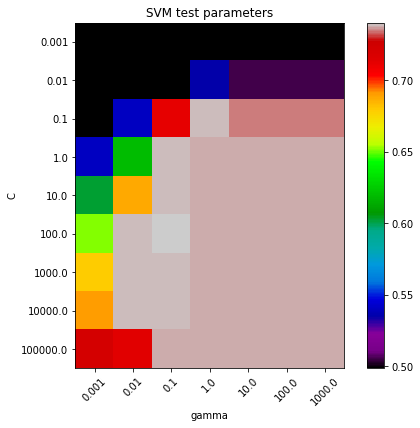
\includegraphics{src/annexes/POC_FindStance_V2/output_24_0.png}
\end{figure}

\textbf{Les valeurs C=100 et gamma=0.1 ont donc été choisi pour réaliser cette SVM, qui fournit finalement un taux d'erreur de $24,49\%$}.

C'est donc cette méthode qui a été implémentée
\subsection{Implémentation d'une SVM}





	\newpage

\newpage

\part{Conclusion}
	\par Durant ce projet l'objectif était de réaliser une analyse de tweet afin d'en extraire le stance, c'est à dire déterminer si l'auteur du tweet était 'POUR', 'CONTRE' ou 'NEUTRE' via à vis d'un sujet donnée. \\

\par Pour cela nous avons donc mis en place plusieurs briques logicielles afin d'arriver à ce résultat. Dans un premier temps nous avons formater les données, puis nous avons commencé par déterminer le sentiment du tweet, c'est à dire si le tweet avait une polarité positive, négative ou neutre. Ensuite l'étape suivante était de déterminer l'opinion toward, c'est à dire déterminer si le tweet faisait référence à un sujet donné de façon direct ou non. L'étape final est donc de déterminer à partir du sentiment et de l'opinion toward, le stance POUR, CONTRE ou NEUTRE. \\

\par Notre choix a été de décomposer les étapes pour arriver au stance afin d'avoir plusieurs systèmes de traitement afin d'être capable d'optimiser chacun des blocs afin de réduire l'erreur finale.  \\

\par Pour la construction de modèle nous avons mis en place des réseaux de neurones, des classifiers et de l'analyse lexicale. Voici les taux de bonne prédiction des meilleurs solutions retenues : \\
\begin{itemize}
	\item Sentiment Analysis : 72.7\% de bonne prédiction par régression logistique.
	\item Opinion Toward : 73,21\%  de bonne prédiction avec un réseau de neurones.
	\item Stance détection : 75,51\% de bonne prédiction avec une SVM.
\end{itemize}

\par Ainsi à partir de données d'apprentissage pour les blocs de machine learning nous avons construit nos modèles et nous avons pu appliquer notre chaîne de traitement à des données de test pour estimer les taux de précision des solutions. Ainsi à partir d'un jeu de données test on obtient un taux de bonne prédiction du stance de 73.619\% ce qui est correcte. \\

\par Nous avons mesuré notre modèle avec le concours international SemEval. Pour cela un script est fourni pour obtenir la métrique du modèle à comparer avec les autres participants, voici ce que l'on obtient : \\

\begin{verbatim}
============
Results
============
FAVOR     precision: 0.4772 recall: 0.3092 f-score: 0.3752
AGAINST   precision: 0.7131 recall: 0.6084 f-score: 0.6566
------------
Macro F: 0.5159
\end{verbatim}

\par Les premiers du concours ont obtenu 0.6910 et les dernier 0.4619, donc notre modèle pourrait être bien amélioré sur les différentes briques afin de réduire les différentes erreurs mais il reste correcte dans l'ensemble. 
	\newpage

\bibliographystyle{plain}
\bibliography{bibliography}

\newpage
\part{Annexes}
	\subsection{POC - Find Stance}
	\label{annexe-stance-detection}	%
% Default to the notebook output style

    


% Inherit from the specified cell style.




    
\documentclass[11pt]{article}

    
    
    \usepackage[T1]{fontenc}
    % Nicer default font (+ math font) than Computer Modern for most use cases
    \usepackage{mathpazo}

    % Basic figure setup, for now with no caption control since it's done
    % automatically by Pandoc (which extracts ![](path) syntax from Markdown).
    \usepackage{graphicx}
    % We will generate all images so they have a width \maxwidth. This means
    % that they will get their normal width if they fit onto the page, but
    % are scaled down if they would overflow the margins.
    \makeatletter
    \def\maxwidth{\ifdim\Gin@nat@width>\linewidth\linewidth
    \else\Gin@nat@width\fi}
    \makeatother
    \let\Oldincludegraphics\includegraphics
    % Set max figure width to be 80% of text width, for now hardcoded.
    \renewcommand{\includegraphics}[1]{\Oldincludegraphics[width=.8\maxwidth]{#1}}
    % Ensure that by default, figures have no caption (until we provide a
    % proper Figure object with a Caption API and a way to capture that
    % in the conversion process - todo).
    \usepackage{caption}
    \DeclareCaptionLabelFormat{nolabel}{}
    \captionsetup{labelformat=nolabel}

    \usepackage{adjustbox} % Used to constrain images to a maximum size 
    \usepackage{xcolor} % Allow colors to be defined
    \usepackage{enumerate} % Needed for markdown enumerations to work
    \usepackage{geometry} % Used to adjust the document margins
    \usepackage{amsmath} % Equations
    \usepackage{amssymb} % Equations
    \usepackage{textcomp} % defines textquotesingle
    % Hack from http://tex.stackexchange.com/a/47451/13684:
    \AtBeginDocument{%
        \def\PYZsq{\textquotesingle}% Upright quotes in Pygmentized code
    }
    \usepackage{upquote} % Upright quotes for verbatim code
    \usepackage{eurosym} % defines \euro
    \usepackage[mathletters]{ucs} % Extended unicode (utf-8) support
    \usepackage[utf8x]{inputenc} % Allow utf-8 characters in the tex document
    \usepackage{fancyvrb} % verbatim replacement that allows latex
    \usepackage{grffile} % extends the file name processing of package graphics 
                         % to support a larger range 
    % The hyperref package gives us a pdf with properly built
    % internal navigation ('pdf bookmarks' for the table of contents,
    % internal cross-reference links, web links for URLs, etc.)
    \usepackage{hyperref}
    \usepackage{longtable} % longtable support required by pandoc >1.10
    \usepackage{booktabs}  % table support for pandoc > 1.12.2
    \usepackage[inline]{enumitem} % IRkernel/repr support (it uses the enumerate* environment)
    \usepackage[normalem]{ulem} % ulem is needed to support strikethroughs (\sout)
                                % normalem makes italics be italics, not underlines
    

    
    
    % Colors for the hyperref package
    \definecolor{urlcolor}{rgb}{0,.145,.698}
    \definecolor{linkcolor}{rgb}{.71,0.21,0.01}
    \definecolor{citecolor}{rgb}{.12,.54,.11}

    % ANSI colors
    \definecolor{ansi-black}{HTML}{3E424D}
    \definecolor{ansi-black-intense}{HTML}{282C36}
    \definecolor{ansi-red}{HTML}{E75C58}
    \definecolor{ansi-red-intense}{HTML}{B22B31}
    \definecolor{ansi-green}{HTML}{00A250}
    \definecolor{ansi-green-intense}{HTML}{007427}
    \definecolor{ansi-yellow}{HTML}{DDB62B}
    \definecolor{ansi-yellow-intense}{HTML}{B27D12}
    \definecolor{ansi-blue}{HTML}{208FFB}
    \definecolor{ansi-blue-intense}{HTML}{0065CA}
    \definecolor{ansi-magenta}{HTML}{D160C4}
    \definecolor{ansi-magenta-intense}{HTML}{A03196}
    \definecolor{ansi-cyan}{HTML}{60C6C8}
    \definecolor{ansi-cyan-intense}{HTML}{258F8F}
    \definecolor{ansi-white}{HTML}{C5C1B4}
    \definecolor{ansi-white-intense}{HTML}{A1A6B2}

    % commands and environments needed by pandoc snippets
    % extracted from the output of `pandoc -s`
    \providecommand{\tightlist}{%
      \setlength{\itemsep}{0pt}\setlength{\parskip}{0pt}}
    \DefineVerbatimEnvironment{Highlighting}{Verbatim}{commandchars=\\\{\}}
    % Add ',fontsize=\small' for more characters per line
    \newenvironment{Shaded}{}{}
    \newcommand{\KeywordTok}[1]{\textcolor[rgb]{0.00,0.44,0.13}{\textbf{{#1}}}}
    \newcommand{\DataTypeTok}[1]{\textcolor[rgb]{0.56,0.13,0.00}{{#1}}}
    \newcommand{\DecValTok}[1]{\textcolor[rgb]{0.25,0.63,0.44}{{#1}}}
    \newcommand{\BaseNTok}[1]{\textcolor[rgb]{0.25,0.63,0.44}{{#1}}}
    \newcommand{\FloatTok}[1]{\textcolor[rgb]{0.25,0.63,0.44}{{#1}}}
    \newcommand{\CharTok}[1]{\textcolor[rgb]{0.25,0.44,0.63}{{#1}}}
    \newcommand{\StringTok}[1]{\textcolor[rgb]{0.25,0.44,0.63}{{#1}}}
    \newcommand{\CommentTok}[1]{\textcolor[rgb]{0.38,0.63,0.69}{\textit{{#1}}}}
    \newcommand{\OtherTok}[1]{\textcolor[rgb]{0.00,0.44,0.13}{{#1}}}
    \newcommand{\AlertTok}[1]{\textcolor[rgb]{1.00,0.00,0.00}{\textbf{{#1}}}}
    \newcommand{\FunctionTok}[1]{\textcolor[rgb]{0.02,0.16,0.49}{{#1}}}
    \newcommand{\RegionMarkerTok}[1]{{#1}}
    \newcommand{\ErrorTok}[1]{\textcolor[rgb]{1.00,0.00,0.00}{\textbf{{#1}}}}
    \newcommand{\NormalTok}[1]{{#1}}
    
    % Additional commands for more recent versions of Pandoc
    \newcommand{\ConstantTok}[1]{\textcolor[rgb]{0.53,0.00,0.00}{{#1}}}
    \newcommand{\SpecialCharTok}[1]{\textcolor[rgb]{0.25,0.44,0.63}{{#1}}}
    \newcommand{\VerbatimStringTok}[1]{\textcolor[rgb]{0.25,0.44,0.63}{{#1}}}
    \newcommand{\SpecialStringTok}[1]{\textcolor[rgb]{0.73,0.40,0.53}{{#1}}}
    \newcommand{\ImportTok}[1]{{#1}}
    \newcommand{\DocumentationTok}[1]{\textcolor[rgb]{0.73,0.13,0.13}{\textit{{#1}}}}
    \newcommand{\AnnotationTok}[1]{\textcolor[rgb]{0.38,0.63,0.69}{\textbf{\textit{{#1}}}}}
    \newcommand{\CommentVarTok}[1]{\textcolor[rgb]{0.38,0.63,0.69}{\textbf{\textit{{#1}}}}}
    \newcommand{\VariableTok}[1]{\textcolor[rgb]{0.10,0.09,0.49}{{#1}}}
    \newcommand{\ControlFlowTok}[1]{\textcolor[rgb]{0.00,0.44,0.13}{\textbf{{#1}}}}
    \newcommand{\OperatorTok}[1]{\textcolor[rgb]{0.40,0.40,0.40}{{#1}}}
    \newcommand{\BuiltInTok}[1]{{#1}}
    \newcommand{\ExtensionTok}[1]{{#1}}
    \newcommand{\PreprocessorTok}[1]{\textcolor[rgb]{0.74,0.48,0.00}{{#1}}}
    \newcommand{\AttributeTok}[1]{\textcolor[rgb]{0.49,0.56,0.16}{{#1}}}
    \newcommand{\InformationTok}[1]{\textcolor[rgb]{0.38,0.63,0.69}{\textbf{\textit{{#1}}}}}
    \newcommand{\WarningTok}[1]{\textcolor[rgb]{0.38,0.63,0.69}{\textbf{\textit{{#1}}}}}
    
    
    % Define a nice break command that doesn't care if a line doesn't already
    % exist.
    \def\br{\hspace*{\fill} \\* }
    % Math Jax compatability definitions
    \def\gt{>}
    \def\lt{<}
    % Document parameters
    \title{POC\_FindStance\_V2}
    
    
    

    % Pygments definitions
    
\makeatletter
\def\PY@reset{\let\PY@it=\relax \let\PY@bf=\relax%
    \let\PY@ul=\relax \let\PY@tc=\relax%
    \let\PY@bc=\relax \let\PY@ff=\relax}
\def\PY@tok#1{\csname PY@tok@#1\endcsname}
\def\PY@toks#1+{\ifx\relax#1\empty\else%
    \PY@tok{#1}\expandafter\PY@toks\fi}
\def\PY@do#1{\PY@bc{\PY@tc{\PY@ul{%
    \PY@it{\PY@bf{\PY@ff{#1}}}}}}}
\def\PY#1#2{\PY@reset\PY@toks#1+\relax+\PY@do{#2}}

\expandafter\def\csname PY@tok@w\endcsname{\def\PY@tc##1{\textcolor[rgb]{0.73,0.73,0.73}{##1}}}
\expandafter\def\csname PY@tok@c\endcsname{\let\PY@it=\textit\def\PY@tc##1{\textcolor[rgb]{0.25,0.50,0.50}{##1}}}
\expandafter\def\csname PY@tok@cp\endcsname{\def\PY@tc##1{\textcolor[rgb]{0.74,0.48,0.00}{##1}}}
\expandafter\def\csname PY@tok@k\endcsname{\let\PY@bf=\textbf\def\PY@tc##1{\textcolor[rgb]{0.00,0.50,0.00}{##1}}}
\expandafter\def\csname PY@tok@kp\endcsname{\def\PY@tc##1{\textcolor[rgb]{0.00,0.50,0.00}{##1}}}
\expandafter\def\csname PY@tok@kt\endcsname{\def\PY@tc##1{\textcolor[rgb]{0.69,0.00,0.25}{##1}}}
\expandafter\def\csname PY@tok@o\endcsname{\def\PY@tc##1{\textcolor[rgb]{0.40,0.40,0.40}{##1}}}
\expandafter\def\csname PY@tok@ow\endcsname{\let\PY@bf=\textbf\def\PY@tc##1{\textcolor[rgb]{0.67,0.13,1.00}{##1}}}
\expandafter\def\csname PY@tok@nb\endcsname{\def\PY@tc##1{\textcolor[rgb]{0.00,0.50,0.00}{##1}}}
\expandafter\def\csname PY@tok@nf\endcsname{\def\PY@tc##1{\textcolor[rgb]{0.00,0.00,1.00}{##1}}}
\expandafter\def\csname PY@tok@nc\endcsname{\let\PY@bf=\textbf\def\PY@tc##1{\textcolor[rgb]{0.00,0.00,1.00}{##1}}}
\expandafter\def\csname PY@tok@nn\endcsname{\let\PY@bf=\textbf\def\PY@tc##1{\textcolor[rgb]{0.00,0.00,1.00}{##1}}}
\expandafter\def\csname PY@tok@ne\endcsname{\let\PY@bf=\textbf\def\PY@tc##1{\textcolor[rgb]{0.82,0.25,0.23}{##1}}}
\expandafter\def\csname PY@tok@nv\endcsname{\def\PY@tc##1{\textcolor[rgb]{0.10,0.09,0.49}{##1}}}
\expandafter\def\csname PY@tok@no\endcsname{\def\PY@tc##1{\textcolor[rgb]{0.53,0.00,0.00}{##1}}}
\expandafter\def\csname PY@tok@nl\endcsname{\def\PY@tc##1{\textcolor[rgb]{0.63,0.63,0.00}{##1}}}
\expandafter\def\csname PY@tok@ni\endcsname{\let\PY@bf=\textbf\def\PY@tc##1{\textcolor[rgb]{0.60,0.60,0.60}{##1}}}
\expandafter\def\csname PY@tok@na\endcsname{\def\PY@tc##1{\textcolor[rgb]{0.49,0.56,0.16}{##1}}}
\expandafter\def\csname PY@tok@nt\endcsname{\let\PY@bf=\textbf\def\PY@tc##1{\textcolor[rgb]{0.00,0.50,0.00}{##1}}}
\expandafter\def\csname PY@tok@nd\endcsname{\def\PY@tc##1{\textcolor[rgb]{0.67,0.13,1.00}{##1}}}
\expandafter\def\csname PY@tok@s\endcsname{\def\PY@tc##1{\textcolor[rgb]{0.73,0.13,0.13}{##1}}}
\expandafter\def\csname PY@tok@sd\endcsname{\let\PY@it=\textit\def\PY@tc##1{\textcolor[rgb]{0.73,0.13,0.13}{##1}}}
\expandafter\def\csname PY@tok@si\endcsname{\let\PY@bf=\textbf\def\PY@tc##1{\textcolor[rgb]{0.73,0.40,0.53}{##1}}}
\expandafter\def\csname PY@tok@se\endcsname{\let\PY@bf=\textbf\def\PY@tc##1{\textcolor[rgb]{0.73,0.40,0.13}{##1}}}
\expandafter\def\csname PY@tok@sr\endcsname{\def\PY@tc##1{\textcolor[rgb]{0.73,0.40,0.53}{##1}}}
\expandafter\def\csname PY@tok@ss\endcsname{\def\PY@tc##1{\textcolor[rgb]{0.10,0.09,0.49}{##1}}}
\expandafter\def\csname PY@tok@sx\endcsname{\def\PY@tc##1{\textcolor[rgb]{0.00,0.50,0.00}{##1}}}
\expandafter\def\csname PY@tok@m\endcsname{\def\PY@tc##1{\textcolor[rgb]{0.40,0.40,0.40}{##1}}}
\expandafter\def\csname PY@tok@gh\endcsname{\let\PY@bf=\textbf\def\PY@tc##1{\textcolor[rgb]{0.00,0.00,0.50}{##1}}}
\expandafter\def\csname PY@tok@gu\endcsname{\let\PY@bf=\textbf\def\PY@tc##1{\textcolor[rgb]{0.50,0.00,0.50}{##1}}}
\expandafter\def\csname PY@tok@gd\endcsname{\def\PY@tc##1{\textcolor[rgb]{0.63,0.00,0.00}{##1}}}
\expandafter\def\csname PY@tok@gi\endcsname{\def\PY@tc##1{\textcolor[rgb]{0.00,0.63,0.00}{##1}}}
\expandafter\def\csname PY@tok@gr\endcsname{\def\PY@tc##1{\textcolor[rgb]{1.00,0.00,0.00}{##1}}}
\expandafter\def\csname PY@tok@ge\endcsname{\let\PY@it=\textit}
\expandafter\def\csname PY@tok@gs\endcsname{\let\PY@bf=\textbf}
\expandafter\def\csname PY@tok@gp\endcsname{\let\PY@bf=\textbf\def\PY@tc##1{\textcolor[rgb]{0.00,0.00,0.50}{##1}}}
\expandafter\def\csname PY@tok@go\endcsname{\def\PY@tc##1{\textcolor[rgb]{0.53,0.53,0.53}{##1}}}
\expandafter\def\csname PY@tok@gt\endcsname{\def\PY@tc##1{\textcolor[rgb]{0.00,0.27,0.87}{##1}}}
\expandafter\def\csname PY@tok@err\endcsname{\def\PY@bc##1{\setlength{\fboxsep}{0pt}\fcolorbox[rgb]{1.00,0.00,0.00}{1,1,1}{\strut ##1}}}
\expandafter\def\csname PY@tok@kc\endcsname{\let\PY@bf=\textbf\def\PY@tc##1{\textcolor[rgb]{0.00,0.50,0.00}{##1}}}
\expandafter\def\csname PY@tok@kd\endcsname{\let\PY@bf=\textbf\def\PY@tc##1{\textcolor[rgb]{0.00,0.50,0.00}{##1}}}
\expandafter\def\csname PY@tok@kn\endcsname{\let\PY@bf=\textbf\def\PY@tc##1{\textcolor[rgb]{0.00,0.50,0.00}{##1}}}
\expandafter\def\csname PY@tok@kr\endcsname{\let\PY@bf=\textbf\def\PY@tc##1{\textcolor[rgb]{0.00,0.50,0.00}{##1}}}
\expandafter\def\csname PY@tok@bp\endcsname{\def\PY@tc##1{\textcolor[rgb]{0.00,0.50,0.00}{##1}}}
\expandafter\def\csname PY@tok@fm\endcsname{\def\PY@tc##1{\textcolor[rgb]{0.00,0.00,1.00}{##1}}}
\expandafter\def\csname PY@tok@vc\endcsname{\def\PY@tc##1{\textcolor[rgb]{0.10,0.09,0.49}{##1}}}
\expandafter\def\csname PY@tok@vg\endcsname{\def\PY@tc##1{\textcolor[rgb]{0.10,0.09,0.49}{##1}}}
\expandafter\def\csname PY@tok@vi\endcsname{\def\PY@tc##1{\textcolor[rgb]{0.10,0.09,0.49}{##1}}}
\expandafter\def\csname PY@tok@vm\endcsname{\def\PY@tc##1{\textcolor[rgb]{0.10,0.09,0.49}{##1}}}
\expandafter\def\csname PY@tok@sa\endcsname{\def\PY@tc##1{\textcolor[rgb]{0.73,0.13,0.13}{##1}}}
\expandafter\def\csname PY@tok@sb\endcsname{\def\PY@tc##1{\textcolor[rgb]{0.73,0.13,0.13}{##1}}}
\expandafter\def\csname PY@tok@sc\endcsname{\def\PY@tc##1{\textcolor[rgb]{0.73,0.13,0.13}{##1}}}
\expandafter\def\csname PY@tok@dl\endcsname{\def\PY@tc##1{\textcolor[rgb]{0.73,0.13,0.13}{##1}}}
\expandafter\def\csname PY@tok@s2\endcsname{\def\PY@tc##1{\textcolor[rgb]{0.73,0.13,0.13}{##1}}}
\expandafter\def\csname PY@tok@sh\endcsname{\def\PY@tc##1{\textcolor[rgb]{0.73,0.13,0.13}{##1}}}
\expandafter\def\csname PY@tok@s1\endcsname{\def\PY@tc##1{\textcolor[rgb]{0.73,0.13,0.13}{##1}}}
\expandafter\def\csname PY@tok@mb\endcsname{\def\PY@tc##1{\textcolor[rgb]{0.40,0.40,0.40}{##1}}}
\expandafter\def\csname PY@tok@mf\endcsname{\def\PY@tc##1{\textcolor[rgb]{0.40,0.40,0.40}{##1}}}
\expandafter\def\csname PY@tok@mh\endcsname{\def\PY@tc##1{\textcolor[rgb]{0.40,0.40,0.40}{##1}}}
\expandafter\def\csname PY@tok@mi\endcsname{\def\PY@tc##1{\textcolor[rgb]{0.40,0.40,0.40}{##1}}}
\expandafter\def\csname PY@tok@il\endcsname{\def\PY@tc##1{\textcolor[rgb]{0.40,0.40,0.40}{##1}}}
\expandafter\def\csname PY@tok@mo\endcsname{\def\PY@tc##1{\textcolor[rgb]{0.40,0.40,0.40}{##1}}}
\expandafter\def\csname PY@tok@ch\endcsname{\let\PY@it=\textit\def\PY@tc##1{\textcolor[rgb]{0.25,0.50,0.50}{##1}}}
\expandafter\def\csname PY@tok@cm\endcsname{\let\PY@it=\textit\def\PY@tc##1{\textcolor[rgb]{0.25,0.50,0.50}{##1}}}
\expandafter\def\csname PY@tok@cpf\endcsname{\let\PY@it=\textit\def\PY@tc##1{\textcolor[rgb]{0.25,0.50,0.50}{##1}}}
\expandafter\def\csname PY@tok@c1\endcsname{\let\PY@it=\textit\def\PY@tc##1{\textcolor[rgb]{0.25,0.50,0.50}{##1}}}
\expandafter\def\csname PY@tok@cs\endcsname{\let\PY@it=\textit\def\PY@tc##1{\textcolor[rgb]{0.25,0.50,0.50}{##1}}}

\def\PYZbs{\char`\\}
\def\PYZus{\char`\_}
\def\PYZob{\char`\{}
\def\PYZcb{\char`\}}
\def\PYZca{\char`\^}
\def\PYZam{\char`\&}
\def\PYZlt{\char`\<}
\def\PYZgt{\char`\>}
\def\PYZsh{\char`\#}
\def\PYZpc{\char`\%}
\def\PYZdl{\char`\$}
\def\PYZhy{\char`\-}
\def\PYZsq{\char`\'}
\def\PYZdq{\char`\"}
\def\PYZti{\char`\~}
% for compatibility with earlier versions
\def\PYZat{@}
\def\PYZlb{[}
\def\PYZrb{]}
\makeatother


    % Exact colors from NB
    \definecolor{incolor}{rgb}{0.0, 0.0, 0.5}
    \definecolor{outcolor}{rgb}{0.545, 0.0, 0.0}



    
    % Prevent overflowing lines due to hard-to-break entities
    \sloppy 
    % Setup hyperref package
    \hypersetup{
      breaklinks=true,  % so long urls are correctly broken across lines
      colorlinks=true,
      urlcolor=urlcolor,
      linkcolor=linkcolor,
      citecolor=citecolor,
      }
    % Slightly bigger margins than the latex defaults
    
    \geometry{verbose,tmargin=1in,bmargin=1in,lmargin=1in,rmargin=1in}
    
    

    \begin{document}
    
    
    \maketitle
    
    

    
    \begin{Verbatim}[commandchars=\\\{\}]
{\color{incolor}In [{\color{incolor}1}]:} \PY{k+kn}{import} \PY{n+nn}{math} \PY{k}{as} \PY{n+nn}{m}
        \PY{k+kn}{import} \PY{n+nn}{numpy} \PY{k}{as} \PY{n+nn}{np}
        \PY{k+kn}{import} \PY{n+nn}{matplotlib}\PY{n+nn}{.}\PY{n+nn}{pyplot} \PY{k}{as} \PY{n+nn}{plt}
        \PY{k+kn}{import} \PY{n+nn}{pandas} \PY{k}{as} \PY{n+nn}{pd}
        \PY{k+kn}{from} \PY{n+nn}{sklearn} \PY{k}{import} \PY{n}{svm}
        \PY{k+kn}{from} \PY{n+nn}{sklearn} \PY{k}{import} \PY{n}{preprocessing}
        \PY{k+kn}{from} \PY{n+nn}{sklearn}\PY{n+nn}{.}\PY{n+nn}{svm} \PY{k}{import} \PY{n}{LinearSVC}
        \PY{k+kn}{from} \PY{n+nn}{sklearn}\PY{n+nn}{.}\PY{n+nn}{preprocessing} \PY{k}{import} \PY{n}{LabelEncoder}
        \PY{k+kn}{from} \PY{n+nn}{sklearn}\PY{n+nn}{.}\PY{n+nn}{model\PYZus{}selection} \PY{k}{import} \PY{n}{train\PYZus{}test\PYZus{}split}
        \PY{k+kn}{from} \PY{n+nn}{sklearn}\PY{n+nn}{.}\PY{n+nn}{naive\PYZus{}bayes} \PY{k}{import} \PY{n}{GaussianNB}
        \PY{k+kn}{from} \PY{n+nn}{sklearn}\PY{n+nn}{.}\PY{n+nn}{neighbors} \PY{k}{import} \PY{n}{KNeighborsClassifier}
        \PY{k+kn}{from} \PY{n+nn}{sklearn}\PY{n+nn}{.}\PY{n+nn}{tree} \PY{k}{import} \PY{n}{DecisionTreeClassifier}
        \PY{k+kn}{import} \PY{n+nn}{warnings}
        \PY{n}{warnings}\PY{o}{.}\PY{n}{filterwarnings}\PY{p}{(}\PY{l+s+s1}{\PYZsq{}}\PY{l+s+s1}{ignore}\PY{l+s+s1}{\PYZsq{}}\PY{p}{)}
        
        \PY{n}{np}\PY{o}{.}\PY{n}{set\PYZus{}printoptions}\PY{p}{(}\PY{n}{threshold}\PY{o}{=}\PY{n}{np}\PY{o}{.}\PY{n}{inf}\PY{p}{)}
\end{Verbatim}


    \section{Chargement des données}\label{chargement-des-donnuxe9es}

    \begin{Verbatim}[commandchars=\\\{\}]
{\color{incolor}In [{\color{incolor}2}]:} \PY{n}{df\PYZus{}train} \PY{o}{=} \PY{n}{pd}\PY{o}{.}\PY{n}{read\PYZus{}csv}\PY{p}{(}\PY{l+s+s1}{\PYZsq{}}\PY{l+s+s1}{./dataset/train\PYZus{}ingrid.csv}\PY{l+s+s1}{\PYZsq{}}\PY{p}{)}
        \PY{n}{df\PYZus{}test} \PY{o}{=} \PY{n}{pd}\PY{o}{.}\PY{n}{read\PYZus{}csv}\PY{p}{(}\PY{l+s+s1}{\PYZsq{}}\PY{l+s+s1}{./dataset/test\PYZus{}ingrid.csv}\PY{l+s+s1}{\PYZsq{}}\PY{p}{)}
\end{Verbatim}


    \subsection{Fusion des données}\label{fusion-des-donnuxe9es}

    \begin{Verbatim}[commandchars=\\\{\}]
{\color{incolor}In [{\color{incolor}3}]:} \PY{n}{target} \PY{o}{=} \PY{n}{np}\PY{o}{.}\PY{n}{hstack}\PY{p}{(}\PY{p}{[}\PY{n}{np}\PY{o}{.}\PY{n}{array}\PY{p}{(}\PY{n}{df\PYZus{}train}\PY{p}{[}\PY{l+s+s1}{\PYZsq{}}\PY{l+s+s1}{Target}\PY{l+s+s1}{\PYZsq{}}\PY{p}{]}\PY{p}{)}\PY{p}{,} \PY{n}{np}\PY{o}{.}\PY{n}{array}\PY{p}{(}\PY{n}{df\PYZus{}test}\PY{p}{[}\PY{l+s+s1}{\PYZsq{}}\PY{l+s+s1}{Target}\PY{l+s+s1}{\PYZsq{}}\PY{p}{]}\PY{p}{)}\PY{p}{]}\PY{p}{)}
        \PY{n}{opinion} \PY{o}{=} \PY{n}{np}\PY{o}{.}\PY{n}{hstack}\PY{p}{(}\PY{p}{[}\PY{n}{np}\PY{o}{.}\PY{n}{array}\PY{p}{(}\PY{n}{df\PYZus{}train}\PY{p}{[}\PY{l+s+s1}{\PYZsq{}}\PY{l+s+s1}{Opinion Towards}\PY{l+s+s1}{\PYZsq{}}\PY{p}{]}\PY{p}{)}\PY{p}{,} \PY{n}{np}\PY{o}{.}\PY{n}{array}\PY{p}{(}\PY{n}{df\PYZus{}test}\PY{p}{[}\PY{l+s+s1}{\PYZsq{}}\PY{l+s+s1}{Opinion Towards}\PY{l+s+s1}{\PYZsq{}}\PY{p}{]}\PY{p}{)}\PY{p}{]}\PY{p}{)}
        \PY{n}{sentiment} \PY{o}{=} \PY{n}{np}\PY{o}{.}\PY{n}{hstack}\PY{p}{(}\PY{p}{[}\PY{n}{np}\PY{o}{.}\PY{n}{array}\PY{p}{(}\PY{n}{df\PYZus{}train}\PY{p}{[}\PY{l+s+s1}{\PYZsq{}}\PY{l+s+s1}{Sentiment}\PY{l+s+s1}{\PYZsq{}}\PY{p}{]}\PY{p}{)}\PY{p}{,} \PY{n}{np}\PY{o}{.}\PY{n}{array}\PY{p}{(}\PY{n}{df\PYZus{}test}\PY{p}{[}\PY{l+s+s1}{\PYZsq{}}\PY{l+s+s1}{Sentiment}\PY{l+s+s1}{\PYZsq{}}\PY{p}{]}\PY{p}{)}\PY{p}{]}\PY{p}{)}
        \PY{n}{stance} \PY{o}{=} \PY{n}{np}\PY{o}{.}\PY{n}{hstack}\PY{p}{(}\PY{p}{[}\PY{n}{np}\PY{o}{.}\PY{n}{array}\PY{p}{(}\PY{n}{df\PYZus{}train}\PY{p}{[}\PY{l+s+s1}{\PYZsq{}}\PY{l+s+s1}{Stance}\PY{l+s+s1}{\PYZsq{}}\PY{p}{]}\PY{p}{)}\PY{p}{,} \PY{n}{np}\PY{o}{.}\PY{n}{array}\PY{p}{(}\PY{n}{df\PYZus{}test}\PY{p}{[}\PY{l+s+s1}{\PYZsq{}}\PY{l+s+s1}{Stance}\PY{l+s+s1}{\PYZsq{}}\PY{p}{]}\PY{p}{)}\PY{p}{]}\PY{p}{)}
\end{Verbatim}


    \subsection{Encodage des labels (passage en
classes)}\label{encodage-des-labels-passage-en-classes}

    \begin{Verbatim}[commandchars=\\\{\}]
{\color{incolor}In [{\color{incolor}4}]:} \PY{n}{lb\PYZus{}target} \PY{o}{=} \PY{n}{preprocessing}\PY{o}{.}\PY{n}{LabelEncoder}\PY{p}{(}\PY{p}{)}
        \PY{n}{target\PYZus{}label} \PY{o}{=} \PY{n}{lb\PYZus{}target}\PY{o}{.}\PY{n}{fit\PYZus{}transform}\PY{p}{(}\PY{n}{target}\PY{p}{)}
        \PY{n}{lb\PYZus{}opinion} \PY{o}{=} \PY{n}{preprocessing}\PY{o}{.}\PY{n}{LabelEncoder}\PY{p}{(}\PY{p}{)}
        \PY{n}{opinion\PYZus{}label} \PY{o}{=} \PY{n}{lb\PYZus{}opinion}\PY{o}{.}\PY{n}{fit\PYZus{}transform}\PY{p}{(}\PY{n}{opinion}\PY{p}{)}
        \PY{n}{lb\PYZus{}sentiment} \PY{o}{=} \PY{n}{preprocessing}\PY{o}{.}\PY{n}{LabelEncoder}\PY{p}{(}\PY{p}{)}
        \PY{n}{sentiment\PYZus{}label} \PY{o}{=} \PY{n}{lb\PYZus{}sentiment}\PY{o}{.}\PY{n}{fit\PYZus{}transform}\PY{p}{(}\PY{n}{sentiment}\PY{p}{)}
        \PY{n}{lb\PYZus{}stance} \PY{o}{=} \PY{n}{preprocessing}\PY{o}{.}\PY{n}{LabelEncoder}\PY{p}{(}\PY{p}{)}
        \PY{n}{stance\PYZus{}label} \PY{o}{=} \PY{n}{lb\PYZus{}stance}\PY{o}{.}\PY{n}{fit\PYZus{}transform}\PY{p}{(}\PY{n}{stance}\PY{p}{)}
\end{Verbatim}


    \subsection{Découpage en ensemble d'apprentissage et de
test}\label{duxe9coupage-en-ensemble-dapprentissage-et-de-test}

    \begin{Verbatim}[commandchars=\\\{\}]
{\color{incolor}In [{\color{incolor}5}]:} \PY{n}{X} \PY{o}{=} \PY{n}{np}\PY{o}{.}\PY{n}{array}\PY{p}{(}\PY{p}{[}\PY{n}{target\PYZus{}label}\PY{p}{,} \PY{n}{opinion\PYZus{}label}\PY{p}{,} \PY{n}{sentiment\PYZus{}label}\PY{p}{]}\PY{p}{)}
        \PY{n}{X} \PY{o}{=} \PY{n}{np}\PY{o}{.}\PY{n}{transpose}\PY{p}{(}\PY{n}{X}\PY{p}{)}
        \PY{n}{X\PYZus{}train}\PY{p}{,} \PY{n}{X\PYZus{}test}\PY{p}{,} \PY{n}{y\PYZus{}train}\PY{p}{,} \PY{n}{y\PYZus{}test}\PY{o}{=} \PY{n}{train\PYZus{}test\PYZus{}split}\PY{p}{(} \PY{n}{X}\PY{p}{,} \PY{n}{stance\PYZus{}label}\PY{p}{,} \PY{n}{test\PYZus{}size}\PY{o}{=}\PY{l+m+mf}{0.15}\PY{p}{,} \PY{n}{random\PYZus{}state}\PY{o}{=}\PY{l+m+mi}{1} \PY{p}{)}
\end{Verbatim}


    \section{Tests de différentes
méthodes}\label{tests-de-diffuxe9rentes-muxe9thodes}

    \subsection{Bayes}\label{bayes}

    \begin{Verbatim}[commandchars=\\\{\}]
{\color{incolor}In [{\color{incolor}6}]:} \PY{n}{model} \PY{o}{=} \PY{n}{GaussianNB}\PY{p}{(}\PY{p}{)}
        \PY{c+c1}{\PYZsh{} Train the model using the training sets }
        \PY{n}{model}\PY{o}{.}\PY{n}{fit}\PY{p}{(}\PY{n}{X\PYZus{}train}\PY{p}{,} \PY{n}{y\PYZus{}train}\PY{p}{)}
        \PY{c+c1}{\PYZsh{}Predict Output }
        \PY{n}{predicted} \PY{o}{=} \PY{n}{model}\PY{o}{.}\PY{n}{predict}\PY{p}{(}\PY{n}{X\PYZus{}test}\PY{p}{)}
        \PY{n}{erreur} \PY{o}{=} \PY{n+nb}{sum}\PY{p}{(}\PY{p}{(}\PY{n}{y\PYZus{}test} \PY{o}{\PYZhy{}} \PY{n}{predicted}\PY{p}{)} \PY{o}{!=} \PY{l+m+mi}{0}\PY{p}{)}\PY{o}{/}\PY{n+nb}{len}\PY{p}{(}\PY{n}{y\PYZus{}test}\PY{p}{)}\PY{o}{*}\PY{l+m+mi}{100}
        \PY{n}{erreur}
\end{Verbatim}


\begin{Verbatim}[commandchars=\\\{\}]
{\color{outcolor}Out[{\color{outcolor}6}]:} 31.737346101231189
\end{Verbatim}
            
    \subsection{Linear SVM}\label{linear-svm}

    \begin{Verbatim}[commandchars=\\\{\}]
{\color{incolor}In [{\color{incolor}7}]:} \PY{n}{clf} \PY{o}{=} \PY{n}{LinearSVC}\PY{p}{(}\PY{n}{random\PYZus{}state}\PY{o}{=}\PY{l+m+mi}{0}\PY{p}{)}
        \PY{n}{clf}\PY{o}{.}\PY{n}{fit}\PY{p}{(}\PY{n}{X\PYZus{}train}\PY{p}{,} \PY{n}{y\PYZus{}train}\PY{p}{)}
        \PY{n}{dec} \PY{o}{=} \PY{n}{clf}\PY{o}{.}\PY{n}{predict}\PY{p}{(}\PY{n}{X\PYZus{}test}\PY{p}{)}
        \PY{n}{erreur} \PY{o}{=} \PY{n+nb}{sum}\PY{p}{(}\PY{p}{(}\PY{n}{y\PYZus{}test} \PY{o}{\PYZhy{}} \PY{n}{dec}\PY{p}{)} \PY{o}{!=} \PY{l+m+mi}{0}\PY{p}{)}\PY{o}{/}\PY{n+nb}{len}\PY{p}{(}\PY{n}{y\PYZus{}test}\PY{p}{)}\PY{o}{*}\PY{l+m+mi}{100}
        \PY{n}{erreur}
\end{Verbatim}


\begin{Verbatim}[commandchars=\\\{\}]
{\color{outcolor}Out[{\color{outcolor}7}]:} 37.61969904240766
\end{Verbatim}
            
    \subsection{SVM}\label{svm}

    \begin{Verbatim}[commandchars=\\\{\}]
{\color{incolor}In [{\color{incolor}8}]:} \PY{n}{clf} \PY{o}{=} \PY{n}{svm}\PY{o}{.}\PY{n}{SVC}\PY{p}{(}\PY{n}{C}\PY{o}{=}\PY{l+m+mi}{100}\PY{p}{,}\PY{n}{gamma}\PY{o}{=}\PY{l+m+mf}{0.001}\PY{p}{)}
        \PY{n}{clf}\PY{o}{.}\PY{n}{fit}\PY{p}{(}\PY{n}{X\PYZus{}train}\PY{p}{,} \PY{n}{y\PYZus{}train}\PY{p}{)}
        \PY{n}{dec} \PY{o}{=} \PY{n}{clf}\PY{o}{.}\PY{n}{predict}\PY{p}{(}\PY{n}{X\PYZus{}test}\PY{p}{)}
        \PY{n}{erreur} \PY{o}{=} \PY{n+nb}{sum}\PY{p}{(}\PY{p}{(}\PY{n}{y\PYZus{}test} \PY{o}{\PYZhy{}} \PY{n}{dec}\PY{p}{)} \PY{o}{!=} \PY{l+m+mi}{0}\PY{p}{)}\PY{o}{/}\PY{n+nb}{len}\PY{p}{(}\PY{n}{y\PYZus{}test}\PY{p}{)}\PY{o}{*}\PY{l+m+mi}{100}
        \PY{n}{erreur}
\end{Verbatim}


\begin{Verbatim}[commandchars=\\\{\}]
{\color{outcolor}Out[{\color{outcolor}8}]:} 33.105335157318741
\end{Verbatim}
            
    \subsection{K plus proches voisins}\label{k-plus-proches-voisins}

    \begin{Verbatim}[commandchars=\\\{\}]
{\color{incolor}In [{\color{incolor}9}]:} \PY{n}{model} \PY{o}{=} \PY{n}{KNeighborsClassifier}\PY{p}{(}\PY{l+m+mi}{4}\PY{p}{)}
        \PY{c+c1}{\PYZsh{} Train the model using the training sets }
        \PY{n}{model}\PY{o}{.}\PY{n}{fit}\PY{p}{(}\PY{n}{X\PYZus{}train}\PY{p}{,} \PY{n}{y\PYZus{}train}\PY{p}{)}
        \PY{c+c1}{\PYZsh{}Predict Output }
        \PY{n}{predicted} \PY{o}{=} \PY{n}{model}\PY{o}{.}\PY{n}{predict}\PY{p}{(}\PY{n}{X\PYZus{}test}\PY{p}{)}
        \PY{n}{erreur} \PY{o}{=} \PY{n+nb}{sum}\PY{p}{(}\PY{p}{(}\PY{n}{y\PYZus{}test} \PY{o}{\PYZhy{}} \PY{n}{predicted}\PY{p}{)} \PY{o}{!=} \PY{l+m+mi}{0}\PY{p}{)}\PY{o}{/}\PY{n+nb}{len}\PY{p}{(}\PY{n}{y\PYZus{}test}\PY{p}{)}\PY{o}{*}\PY{l+m+mi}{100}
        \PY{n}{erreur}
\end{Verbatim}


\begin{Verbatim}[commandchars=\\\{\}]
{\color{outcolor}Out[{\color{outcolor}9}]:} 34.473324213406293
\end{Verbatim}
            
    \subsection{Arbre de décision}\label{arbre-de-duxe9cision}

    \begin{Verbatim}[commandchars=\\\{\}]
{\color{incolor}In [{\color{incolor}10}]:} \PY{n}{model} \PY{o}{=} \PY{n}{DecisionTreeClassifier}\PY{p}{(}\PY{n}{max\PYZus{}depth}\PY{o}{=}\PY{l+m+mi}{5}\PY{p}{)}
         \PY{c+c1}{\PYZsh{} Train the model using the training sets }
         \PY{n}{model}\PY{o}{.}\PY{n}{fit}\PY{p}{(}\PY{n}{X\PYZus{}train}\PY{p}{,} \PY{n}{y\PYZus{}train}\PY{p}{)}
         \PY{c+c1}{\PYZsh{}Predict Output }
         \PY{n}{predicted} \PY{o}{=} \PY{n}{model}\PY{o}{.}\PY{n}{predict}\PY{p}{(}\PY{n}{X\PYZus{}test}\PY{p}{)}
         \PY{n}{erreur} \PY{o}{=} \PY{n+nb}{sum}\PY{p}{(}\PY{p}{(}\PY{n}{y\PYZus{}test} \PY{o}{\PYZhy{}} \PY{n}{predicted}\PY{p}{)} \PY{o}{!=} \PY{l+m+mi}{0}\PY{p}{)}\PY{o}{/}\PY{n+nb}{len}\PY{p}{(}\PY{n}{y\PYZus{}test}\PY{p}{)}\PY{o}{*}\PY{l+m+mi}{100}
         \PY{n}{erreur}
\end{Verbatim}


\begin{Verbatim}[commandchars=\\\{\}]
{\color{outcolor}Out[{\color{outcolor}10}]:} 24.48700410396717
\end{Verbatim}
            
    \section{Test paramètres SVM}\label{test-paramuxe8tres-svm}

    \begin{Verbatim}[commandchars=\\\{\}]
{\color{incolor}In [{\color{incolor}21}]:} \PY{n}{clf} \PY{o}{=} \PY{n}{svm}\PY{o}{.}\PY{n}{SVC}\PY{p}{(}\PY{n}{kernel}\PY{o}{=}\PY{l+s+s1}{\PYZsq{}}\PY{l+s+s1}{linear}\PY{l+s+s1}{\PYZsq{}}\PY{p}{,} \PY{n}{C}\PY{o}{=}\PY{l+m+mi}{100}\PY{p}{,}\PY{n}{gamma}\PY{o}{=}\PY{l+m+mf}{0.001}\PY{p}{)}
         \PY{n}{clf}\PY{o}{.}\PY{n}{fit}\PY{p}{(}\PY{n}{X\PYZus{}train}\PY{p}{,} \PY{n}{y\PYZus{}train}\PY{p}{)}
         \PY{n}{dec} \PY{o}{=} \PY{n}{clf}\PY{o}{.}\PY{n}{predict}\PY{p}{(}\PY{n}{X\PYZus{}test}\PY{p}{)}
         \PY{n}{erreur} \PY{o}{=} \PY{n+nb}{sum}\PY{p}{(}\PY{p}{(}\PY{n}{y\PYZus{}test} \PY{o}{\PYZhy{}} \PY{n}{dec}\PY{p}{)} \PY{o}{!=} \PY{l+m+mi}{0}\PY{p}{)}\PY{o}{/}\PY{n+nb}{len}\PY{p}{(}\PY{n}{y\PYZus{}test}\PY{p}{)}\PY{o}{*}\PY{l+m+mi}{100}
         \PY{n}{erreur}
\end{Verbatim}


\begin{Verbatim}[commandchars=\\\{\}]
{\color{outcolor}Out[{\color{outcolor}21}]:} 34.610123119015043
\end{Verbatim}
            
    \begin{Verbatim}[commandchars=\\\{\}]
{\color{incolor}In [{\color{incolor}22}]:} \PY{n}{clf} \PY{o}{=} \PY{n}{svm}\PY{o}{.}\PY{n}{SVC}\PY{p}{(}\PY{n}{kernel}\PY{o}{=}\PY{l+s+s1}{\PYZsq{}}\PY{l+s+s1}{rbf}\PY{l+s+s1}{\PYZsq{}}\PY{p}{,} \PY{n}{C}\PY{o}{=}\PY{l+m+mi}{100}\PY{p}{,}\PY{n}{gamma}\PY{o}{=}\PY{l+m+mf}{0.001}\PY{p}{)}
         \PY{n}{clf}\PY{o}{.}\PY{n}{fit}\PY{p}{(}\PY{n}{X\PYZus{}train}\PY{p}{,} \PY{n}{y\PYZus{}train}\PY{p}{)}
         \PY{n}{dec} \PY{o}{=} \PY{n}{clf}\PY{o}{.}\PY{n}{predict}\PY{p}{(}\PY{n}{X\PYZus{}test}\PY{p}{)}
         \PY{n}{erreur} \PY{o}{=} \PY{n+nb}{sum}\PY{p}{(}\PY{p}{(}\PY{n}{y\PYZus{}test} \PY{o}{\PYZhy{}} \PY{n}{dec}\PY{p}{)} \PY{o}{!=} \PY{l+m+mi}{0}\PY{p}{)}\PY{o}{/}\PY{n+nb}{len}\PY{p}{(}\PY{n}{y\PYZus{}test}\PY{p}{)}\PY{o}{*}\PY{l+m+mi}{100}
         \PY{n}{erreur}
\end{Verbatim}


\begin{Verbatim}[commandchars=\\\{\}]
{\color{outcolor}Out[{\color{outcolor}22}]:} 33.105335157318741
\end{Verbatim}
            
    \begin{Verbatim}[commandchars=\\\{\}]
{\color{incolor}In [{\color{incolor}27}]:} \PY{k+kn}{from} \PY{n+nn}{sklearn}\PY{n+nn}{.}\PY{n+nn}{grid\PYZus{}search} \PY{k}{import} \PY{n}{GridSearchCV}
         \PY{k+kn}{from} \PY{n+nn}{sklearn}\PY{n+nn}{.}\PY{n+nn}{cross\PYZus{}validation} \PY{k}{import} \PY{n}{StratifiedKFold}
         
         \PY{n}{C\PYZus{}range} \PY{o}{=} \PY{l+m+mf}{10.} \PY{o}{*}\PY{o}{*} \PY{n}{np}\PY{o}{.}\PY{n}{arange}\PY{p}{(}\PY{o}{\PYZhy{}}\PY{l+m+mi}{3}\PY{p}{,} \PY{l+m+mi}{6}\PY{p}{)}
         \PY{n}{gamma\PYZus{}range} \PY{o}{=} \PY{l+m+mf}{10.} \PY{o}{*}\PY{o}{*} \PY{n}{np}\PY{o}{.}\PY{n}{arange}\PY{p}{(}\PY{o}{\PYZhy{}}\PY{l+m+mi}{5}\PY{p}{,} \PY{l+m+mi}{4}\PY{p}{)}
         \PY{n}{param\PYZus{}grid} \PY{o}{=} \PY{n+nb}{dict}\PY{p}{(}\PY{n}{gamma}\PY{o}{=}\PY{n}{gamma\PYZus{}range}\PY{p}{,} \PY{n}{C}\PY{o}{=}\PY{n}{C\PYZus{}range}\PY{p}{)}
         \PY{n}{grid} \PY{o}{=} \PY{n}{GridSearchCV}\PY{p}{(}\PY{n}{svm}\PY{o}{.}\PY{n}{SVC}\PY{p}{(}\PY{p}{)}\PY{p}{,} \PY{n}{param\PYZus{}grid}\PY{o}{=}\PY{n}{param\PYZus{}grid}\PY{p}{,} \PY{n}{cv}\PY{o}{=}\PY{n}{StratifiedKFold}\PY{p}{(}\PY{n}{y}\PY{o}{=}\PY{n}{y\PYZus{}train}\PY{p}{)}\PY{p}{)}
         \PY{n}{grid}\PY{o}{.}\PY{n}{fit}\PY{p}{(}\PY{n}{X\PYZus{}train}\PY{p}{,} \PY{n}{y\PYZus{}train}\PY{p}{)}
         
         \PY{n+nb}{print}\PY{p}{(}\PY{l+s+s2}{\PYZdq{}}\PY{l+s+s2}{The best classifier is: }\PY{l+s+s2}{\PYZdq{}}\PY{p}{,} \PY{n}{grid}\PY{o}{.}\PY{n}{best\PYZus{}estimator\PYZus{}}\PY{p}{)}
\end{Verbatim}


    \begin{Verbatim}[commandchars=\\\{\}]
The best classifier is:  SVC(C=100.0, cache\_size=200, class\_weight=None, coef0=0.0,
  decision\_function\_shape='ovr', degree=3, gamma=0.10000000000000001,
  kernel='rbf', max\_iter=-1, probability=False, random\_state=None,
  shrinking=True, tol=0.001, verbose=False)

    \end{Verbatim}

    \begin{Verbatim}[commandchars=\\\{\}]
{\color{incolor}In [{\color{incolor}26}]:} \PY{k+kn}{import} \PY{n+nn}{pylab} \PY{k}{as} \PY{n+nn}{pl}
         \PY{c+c1}{\PYZsh{} plot the scores of the grid}
         \PY{c+c1}{\PYZsh{} grid\PYZus{}scores\PYZus{} contains parameter settings and scores}
         \PY{n}{score\PYZus{}dict} \PY{o}{=} \PY{n}{grid}\PY{o}{.}\PY{n}{grid\PYZus{}scores\PYZus{}}
         
         \PY{c+c1}{\PYZsh{} We extract just the scores}
         \PY{n}{scores} \PY{o}{=} \PY{p}{[}\PY{n}{x}\PY{p}{[}\PY{l+m+mi}{1}\PY{p}{]} \PY{k}{for} \PY{n}{x} \PY{o+ow}{in} \PY{n}{score\PYZus{}dict}\PY{p}{]}
         \PY{n}{scores} \PY{o}{=} \PY{n}{np}\PY{o}{.}\PY{n}{array}\PY{p}{(}\PY{n}{scores}\PY{p}{)}\PY{o}{.}\PY{n}{reshape}\PY{p}{(}\PY{n+nb}{len}\PY{p}{(}\PY{n}{C\PYZus{}range}\PY{p}{)}\PY{p}{,} \PY{n+nb}{len}\PY{p}{(}\PY{n}{gamma\PYZus{}range}\PY{p}{)}\PY{p}{)}
         
         \PY{c+c1}{\PYZsh{} Make a nice figure}
         \PY{n}{pl}\PY{o}{.}\PY{n}{figure}\PY{p}{(}\PY{n}{figsize}\PY{o}{=}\PY{p}{(}\PY{l+m+mi}{8}\PY{p}{,} \PY{l+m+mi}{6}\PY{p}{)}\PY{p}{)}
         \PY{n}{pl}\PY{o}{.}\PY{n}{subplots\PYZus{}adjust}\PY{p}{(}\PY{n}{left}\PY{o}{=}\PY{l+m+mf}{0.15}\PY{p}{,} \PY{n}{right}\PY{o}{=}\PY{l+m+mf}{0.95}\PY{p}{,} \PY{n}{bottom}\PY{o}{=}\PY{l+m+mf}{0.15}\PY{p}{,} \PY{n}{top}\PY{o}{=}\PY{l+m+mf}{0.95}\PY{p}{)}
         \PY{n}{pl}\PY{o}{.}\PY{n}{imshow}\PY{p}{(}\PY{n}{scores}\PY{p}{,} \PY{n}{interpolation}\PY{o}{=}\PY{l+s+s1}{\PYZsq{}}\PY{l+s+s1}{nearest}\PY{l+s+s1}{\PYZsq{}}\PY{p}{,} \PY{n}{cmap}\PY{o}{=}\PY{n}{pl}\PY{o}{.}\PY{n}{cm}\PY{o}{.}\PY{n}{spectral}\PY{p}{)}
         \PY{n}{pl}\PY{o}{.}\PY{n}{xlabel}\PY{p}{(}\PY{l+s+s1}{\PYZsq{}}\PY{l+s+s1}{gamma}\PY{l+s+s1}{\PYZsq{}}\PY{p}{)}
         \PY{n}{pl}\PY{o}{.}\PY{n}{ylabel}\PY{p}{(}\PY{l+s+s1}{\PYZsq{}}\PY{l+s+s1}{C}\PY{l+s+s1}{\PYZsq{}}\PY{p}{)}
         \PY{n}{pl}\PY{o}{.}\PY{n}{title}\PY{p}{(}\PY{l+s+s1}{\PYZsq{}}\PY{l+s+s1}{SVM test parameters}\PY{l+s+s1}{\PYZsq{}}\PY{p}{)}
         \PY{n}{pl}\PY{o}{.}\PY{n}{colorbar}\PY{p}{(}\PY{p}{)}
         \PY{n}{pl}\PY{o}{.}\PY{n}{xticks}\PY{p}{(}\PY{n}{np}\PY{o}{.}\PY{n}{arange}\PY{p}{(}\PY{n+nb}{len}\PY{p}{(}\PY{n}{gamma\PYZus{}range}\PY{p}{)}\PY{p}{)}\PY{p}{,} \PY{n}{gamma\PYZus{}range}\PY{p}{,} \PY{n}{rotation}\PY{o}{=}\PY{l+m+mi}{45}\PY{p}{)}
         \PY{n}{pl}\PY{o}{.}\PY{n}{yticks}\PY{p}{(}\PY{n}{np}\PY{o}{.}\PY{n}{arange}\PY{p}{(}\PY{n+nb}{len}\PY{p}{(}\PY{n}{C\PYZus{}range}\PY{p}{)}\PY{p}{)}\PY{p}{,} \PY{n}{C\PYZus{}range}\PY{p}{)}
         \PY{n}{pl}\PY{o}{.}\PY{n}{show}\PY{p}{(}\PY{p}{)}
\end{Verbatim}


    \begin{center}
    \adjustimage{max size={0.9\linewidth}{0.9\paperheight}}{output_24_0.png}
    \end{center}
    { \hspace*{\fill} \\}
    
    \begin{Verbatim}[commandchars=\\\{\}]
{\color{incolor}In [{\color{incolor}23}]:} \PY{n}{clf} \PY{o}{=} \PY{n}{svm}\PY{o}{.}\PY{n}{SVC}\PY{p}{(}\PY{n}{kernel}\PY{o}{=}\PY{l+s+s1}{\PYZsq{}}\PY{l+s+s1}{rbf}\PY{l+s+s1}{\PYZsq{}}\PY{p}{,} \PY{n}{C}\PY{o}{=}\PY{l+m+mi}{100}\PY{p}{,}\PY{n}{gamma}\PY{o}{=}\PY{l+m+mf}{0.1}\PY{p}{)}
         \PY{n}{clf}\PY{o}{.}\PY{n}{fit}\PY{p}{(}\PY{n}{X\PYZus{}train}\PY{p}{,} \PY{n}{y\PYZus{}train}\PY{p}{)}
         \PY{n}{dec} \PY{o}{=} \PY{n}{clf}\PY{o}{.}\PY{n}{predict}\PY{p}{(}\PY{n}{X\PYZus{}test}\PY{p}{)}
         \PY{n}{erreur} \PY{o}{=} \PY{n+nb}{sum}\PY{p}{(}\PY{p}{(}\PY{n}{y\PYZus{}test} \PY{o}{\PYZhy{}} \PY{n}{dec}\PY{p}{)} \PY{o}{!=} \PY{l+m+mi}{0}\PY{p}{)}\PY{o}{/}\PY{n+nb}{len}\PY{p}{(}\PY{n}{y\PYZus{}test}\PY{p}{)}\PY{o}{*}\PY{l+m+mi}{100}
         \PY{n}{erreur}
\end{Verbatim}


\begin{Verbatim}[commandchars=\\\{\}]
{\color{outcolor}Out[{\color{outcolor}23}]:} 24.48700410396717
\end{Verbatim}
            

    % Add a bibliography block to the postdoc
    
    
    
    \end{document}

	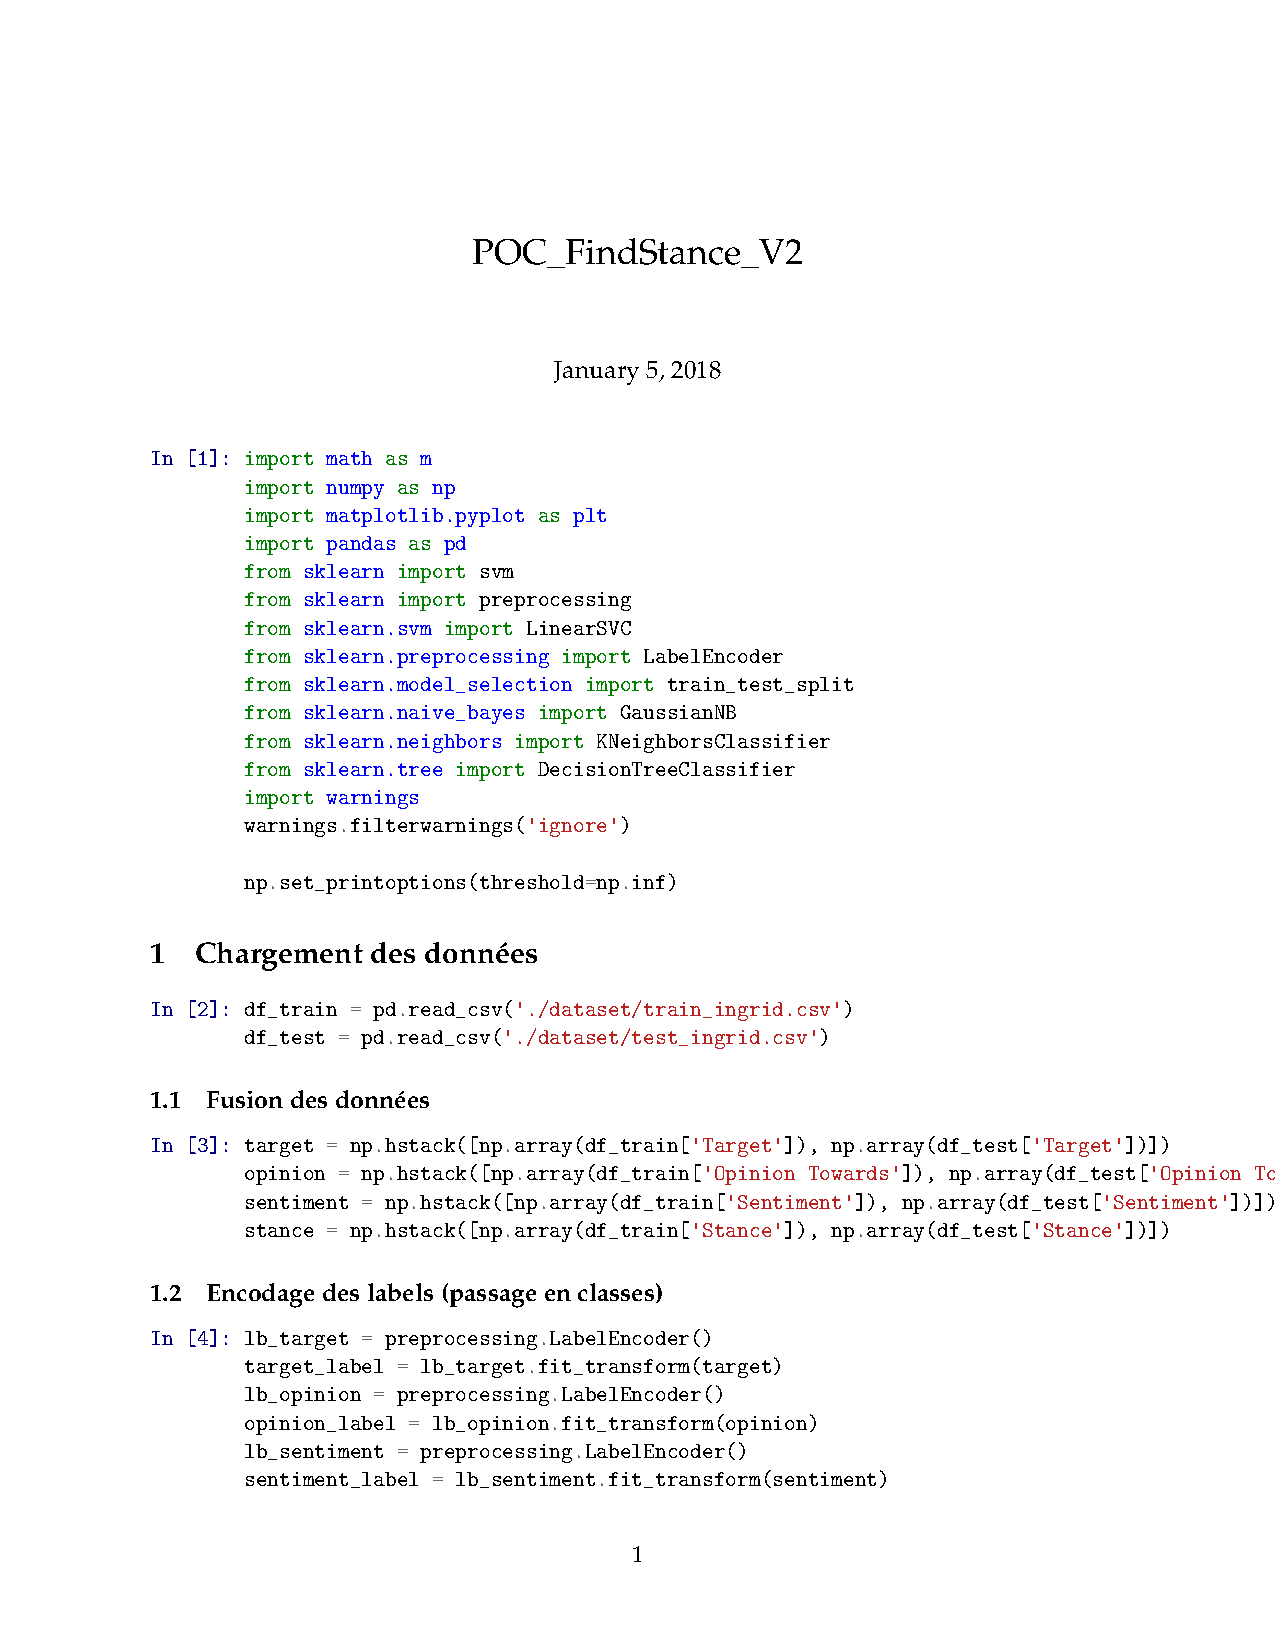
\includepdf[pages={1,2,3,4,5}]{src/annexes/POC_FindStance_V2/POC_FindStance_V2.pdf}
\end{document}
